\documentclass[../SOP.tex]{standalone}

\usepackage{tikz}

\def\layersep{1.5cm}

\begin{document}
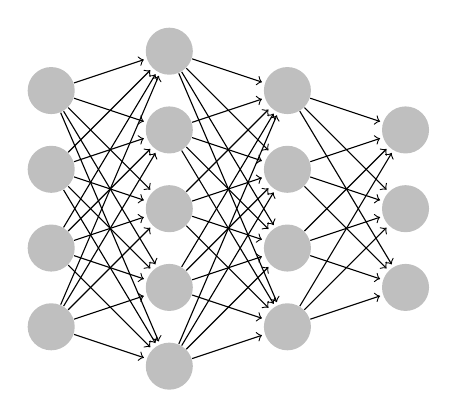
\begin{tikzpicture}[shorten >=1pt,->,draw=black,node distance=\layersep]
  \tikzstyle{every pin edge}=[<-, shorten <= 1pt]
  \tikzstyle{neuron}=[circle,fill=black!25,minimum size=17pt,inner sep=0pt]
  \tikzstyle{annot} = [text width=4em, text centered]

  \foreach \name / \y in {1,...,4}
    \node[neuron] (I-\name) at (0,-\y) {};

  \foreach \name / \y in {1,...,5}
  \path[yshift=0.5cm]
    node[neuron] (Ha-\name) at (\layersep,-\y) {};

  \foreach \name / \y in {1,...,4}
    \node[neuron] (Hb-\name) at (2*\layersep,-\y) {};

  \foreach \name / \y in {1,...,3}
    \path[yshift=-0.5cm]
    node[neuron] (O-\name) at (3*\layersep,-\y) {};

    \foreach \source in {1,...,4}
      \foreach \dest in {1,...,5}
        \path (I-\source) edge (Ha-\dest);

    \foreach \source in {1,...,5}
      \foreach \dest in {1,...,4}
        \path (Ha-\source) edge (Hb-\dest);

    \foreach \source in {1,...,4}
      \foreach \dest in {1,...,3}
        \path (Hb-\source) edge (O-\dest);

    %\node[annot, above of=Ha-1, node distance=1cm] (h1) {Skjult lag 1};
    %\node[annot, right of=h1] (h2) {Skjult lag 2};
    %\node[annot, right of=h2] (o) {Output lag};
    %\node[annot, left of=h1] (i) {Input lag};

\end{tikzpicture}
\end{document}
